\documentclass[10pt,a4paper]{article}
\usepackage[utf8]{inputenc}
\usepackage{amsmath}
\usepackage{amsfonts}
\usepackage{amssymb}
\usepackage{url}
\usepackage{tikz}
\usepackage[slovak]{babel}
\usepackage[margin=1in]{geometry}
\usepackage[american voltages,american currents,european resistors]{circuitikz}
\ctikzset{v/.append style={/tikz/european voltages}}

\begin{document}
\begin{titlepage}

% \vspace*{1cm}
\begin{figure}[!h]
  \centering
  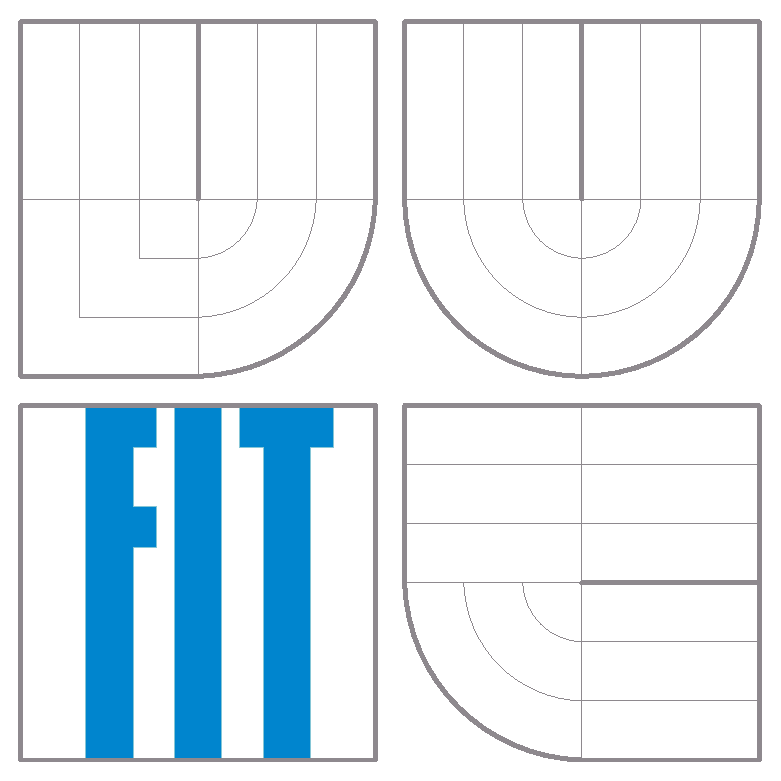
\includegraphics[height=5cm]{img/logo}
\end{figure}

\vfill

\begin{center}
\begin{Large}
Téoria obvodov\\
\end{Large}
\bigskip
\begin{Huge}
Semestrálny projekt\\
\end{Huge}
\end{center}

\vfill

\begin{center}
\begin{Large}
\today
\end{Large}
\end{center}

\vfill

\begin{flushleft}
\begin{large}
\begin{tabular}{ll}
Autor: 
 & Viktor Jančík, \url{xjanci09@stud.fit.vutbr.cz} \\
 & Fakulta Informačních Technologií \\
 & Vysoké Učení Technické v~Brně \\
\end{tabular}
\end{large}
\end{flushleft}
\end{titlepage}

 
\tableofcontents
\pagebreak

\section{Príklad 1}
\subsection{Zadanie}

Stanovte napätie $U_{R7}$ a prúd $I_{R7}$. Použite metódu postupného zjednodušovania obvodu.
\\ \\
\begin{tabular}{|c|c|c|c|c|c|c|c|c|c|}
\hline sk. & U [V] & $R_1$ [$\Omega$] & $R_2$ [$\Omega$] & $R_3$ [$\Omega$] & $R_4$ [$\Omega$] & $R_5$ [$\Omega$] & $R_6$ [$\Omega$] & $R_7$ [$\Omega$] & $R_8$ [$\Omega$]\\
\hline D & 105 & 420 & 980 & 330 & 280 & 310 & 710 & 240 & 200\\
\hline
\end{tabular}

\vspace{10mm}

\begin{tikzpicture}
    \begin{circuitikz}
      \draw (0,0)
      to[V,v^<=$U$] (0,4) % The voltage source
      to[R=$R_1$] (2,4);
      \draw (2,4)
      to [R=$R_2$] (4,4)
      to [R=$R_4$] (4,2)
      to [R=$R_3$] (2,2)
      to [short] (2,4);
      \draw (4,4)
      to [short] (4,5)
      to [R=$R_5$] (6,5)
      to [short] (6,4)
      to [R=$R_6$] (4,4);
      \draw (6,4)
      to [short] (6,2)
      to [R=$R_7$] (4,2);
      \draw (4,2) to[R,i_>=$I_{R7}$,v^>=$U_{R7}$] (6,2);
      \draw (6,2)
      to [short] (6,0)
      to [short] (4,0)
      to [R=$R_8$] (0,0);
    \end{circuitikz}
\end{tikzpicture}
\subsection{Riešenie}

Transformácia $R_2$, $R_3$ a $R_4$ na $R_{23}$, $R_{24}$ a $R_{34}$:
\\
\begin{equation*}
R_{23} = \frac{R_2*R_3}{R_2+R_3+R_4} \hspace{1cm} R_{24} = \frac{R_2*R_4}{R_2+R_3+R_4} \hspace{1cm} R_{34} = \frac{R_3*R_4}{R_2+R_3+R_4}
\end{equation*}
\\
Spojenie $R_5$ a $R_6$:
\\
\begin{equation*}
R_{5,6} = \frac{R_5*R_6}{R_5+R_6}
\end{equation*}
\\
Celkový odpor obvodu:
\\
\begin{equation*}
R = R_1 + R_{23} + \frac{(R_{24}+R_{5,6})*(R_{34}+R_7)}{R_{24}+R_{5,6}+R_{34}+R_7} + R_8
\end{equation*}
\\
Celkový prúd v obvode:
\\
\begin{equation*}
I = \frac{U}{R}
\end{equation*}
\\
Prúd na vetve s resistormi $R_{34}$ a $R_7$:
\\
\begin{equation*}
I_{R_7} = \frac{R_{24}+R_{5,6}}{R_{24}+R_{5,6}+R_{34}+R_7}*I
\end{equation*}
\\
Napätie na resistore $R_7$:
\\
\begin{equation*}
U_{R7} = I_{R_7}*R_7
\end{equation*}

\subsection{Výsledky}

$I_{R_7} = 0.0599 A \hspace{1cm} U_{R_7} = 14.3708 V$

\section{Príklad 2}
\subsection{Zadanie}
Stanovte napätie $U_{R3}$ a prúd $I_{R3}$. Použite metódu Theveninovej vety.
\\ \\
\begin{tabular}{|c|c|c|c|c|c|c|c|}
\hline sk. & $U$ [V] & $R_1$ [$\Omega$] & $R_2$ [$\Omega$] & $R_3$ [$\Omega$] & $R_4$ [$\Omega$] & $R_5$ [$\Omega$] & $R_6$ [$\Omega$]\\
\hline A & 50 & 525 & 620 & 	210 & 530 & 130 & 150\\
\hline
\end{tabular}

\vspace{10mm}

\begin{tikzpicture}
    \begin{circuitikz}
    		\draw (0,0)
    		to [short] (0,1)
    		to [V,v^<=$U$] (0,4)
    		to [short] (1,4)
    		to [R=$R_1$] (3,4)
    		to [R=$R_4$] (5,4)
    		to [short] (5,2)
    		to [R=$R_5$] (3,2)
    		to [R=$R_2$] (1,2)
    		to [short] (1,4);
    		\draw (5,2)
    		to [short] (5,0)
    		to [R=$R_6$] (1,0)
    		to [short] (0,0);
    		\draw (3,4)
    		to [R=$R_3$,i^>=$I_{R3}$,v_>=$U_{R3}$] (3,2);
    \end{circuitikz}
\end{tikzpicture}

\subsection{Riešenie}

Transformácia $R_1$, $R_4$ a $R_6$ na $R_{14}$, $R_{16}$ a $R_{46}$:

\begin{equation*}
R_{14} = \frac{R_1*R_4}{R_1+R_4+R_6} \hspace{1cm} R_{16} = \frac{R_1*R_6}{R_1+R_4+R_6} \hspace{1cm} R_{46} = \frac{R_4*R_6}{R_1+R_4+R_6}
\end{equation*}
\\
Theveninov ekvivalentný odpor na svorkách odporu $R_3$:
\\
\begin{equation*}
R_i = R_{14} + \frac{(R_{16}+R_2)*(R_{46}+R_5)}{R_{16}+R_2+R_{46}+R_5}
\end{equation*}
\\
Celkový odpor obvodu bez odporu $R_3$:
\\
\begin{equation*}
R = \frac{(R_1+R_4)*(R_2+R_5)}{R_1+R_4+R_2+R_5} + R_6
\end{equation*}
\\
Celkový prúd v obvode bez odporu $R_3$:
\\
\begin{equation*}
I = \frac{U}{R}
\end{equation*}
\\
Prúdy na vetvách s odpormi $R_1$, $R_4$ a $R_2$, $R_5$:
\\
\begin{equation*}
I_{R_1,R_4} = \frac{U}{R_1+R_4} \hspace{1cm} I_{R_2,R_5} = \frac{U}{R_2+R_5}
\end{equation*}
\\
Theveninové ekvivalentné napätie obvodu na svorkách rezistora $R_3$:
\\
\begin{equation*}
U_i = U_{R_2} - U_{R_1} = I_{R_2,R_5}*R_2 - I_{R_1,R_4}*R_1
\end{equation*}
\\
Prúd, ktorý prechádza rezistorom $R_3$:
\\
\begin{equation*}
I_{R3} = \frac{U_i}{R_i+R_3}
\end{equation*}
\\
Napätie na rezistore $R_3$:
\\
\begin{equation*}
U_{R3} = I_{R3}*R_3
\end{equation*}

\subsection{Výsledky}

$I_{R3} = 0.0207 A \hspace{1cm} U_{R3} = 4.3385 V$

\section{Príklad 3}
\subsection{Zadanie}

Stanovte napätie $U_{R5}$ a prúd $I_{R5}$. Použite metódu uzlových napätí ($U_A$, $U_B$, $U_C$).
\\ \\
\begin{tabular}{|c|c|c|c|c|c|c|c|c|c|c|}
\hline sk. & $U_1$ [V] & $U_2$ [V] & $I$ [A] & $R_1$ [$\Omega$] & $R_2$ [$\Omega$] & $R_3$ [$\Omega$] & $R_4$ [$\Omega$] & $R_5$ [$\Omega$] & $R_6$ [$\Omega$]\\
\hline G & 160 & 105 & 0.45 & 460 & 410 & 535 & 330 & 290 & 210 \\
\hline
\end{tabular}

\vspace{10mm}

\begin{tikzpicture}
	\begin{circuitikz}
		\draw (0,0)
		to [short] (0,1)
		to [V,v^<=$U_1$] (0,5)
		to [R=$R_1$] (2,5)
		to [short] (2,7)
		to [I,i=$I$] (6,7)
		to [short] (6,5)
		to [short] (7,5)
		to [R=$R_6$] (9,5)
		to [open] (9,1)
		to [short] (9,0)
		to [short] (6,0)
		to [R=$R_4$,v_>=$U_C$] (2,0)
		to [short] (0,0);
		\draw (9,1)
		to [V,v^<=$U_2$] (9,5);
		\draw (2,0)
		to [R=$R_2$] (2,2)
		to [short] (2,5)
		to [R=$R_3$] (6,5)
		to [short,i^>=$I_{R5}$] (6,2)
		to [R=$R_5$,v_>=$U_{R5}$] (6,0);
		\draw (2,5)
		to [open,v^>=$U_A$] (2,0);
		\draw (6,5)
		to [open,v^>=$U_B$] (2,0);
	\end{circuitikz}
\end{tikzpicture}

\subsection{Riešenie}

Rovnice pre uzly A, B a C (sústava troch rovníc s troma neznámymi):

\begin{equation*}
A: \hspace{1cm} \frac{U_1-U_A}{R_1} = \frac{U_2}{R_2} + \frac{U_A-U_B}{R_3} + I
\end{equation*}
\\
\begin{equation*}
B: \hspace{1cm} \frac{U_B-U_C}{R_5} = \frac{U_A-U_B}{R_3} + \frac{U_C+U_2-U_B}{R_6} + I
\end{equation*}
\\
\begin{equation*}
C: \hspace{1cm} \frac{U_B-U_C}{R_5} = \frac{U_C}{R_4} + \frac{U_C+U_2-U_B}{R_6}
\end{equation*}
\\
Napätie na rezistore $R_5$:
\\
\begin{equation*}
U_{R5} = U_B - U_C
\end{equation*}
\\
Prúd na rezistore $R_5$:
\\
\begin{equation*}
I_{R5} = \frac{U_{R5}}{R_5}
\end{equation*}

\subsection{Výsledky}

$U_{R5} = 86.7310 V \hspace{1cm} I_{R5} = 0.2991 A$

\section{Príklad 4}
\subsection{Zadanie}

Pre napájacie napätie platí: $u = U * sin( 2 \pi f t )$.\\
Vo vzťahu pre napätie $u_{L_2} = U_{L_2} * sin(2 \pi f t + \varphi_{L_2})$ určte $|U_{L_2}|$ a  $\varphi_{L_2}$. Použite metódu zjednodušovania obvodov.\\ \\
Pozn: Pomocný "smer šípky napájacieho zdroja platí pre špeciálny časový okamih ($t = \frac{\pi}{2 \omega}$)."
\\ \\
\begin{tabular}{|c|c|c|c|c|c|c|c|c|c|}
\hline sk. & $U$ [V] & $R_1$ [$\Omega$] & $R_2$ [$\Omega$] & $R_3$ [$\Omega$] & $L_1$ [mH] & $L_2$ [mH] & $C_1$ [$\mu$F] & $C_2$ [$\mu$F] & $f$ [Hz]\\
\hline D & 50 & 190 & 180 & 	220 & 420 & 270 & 120 & 205 & 90 \\
\hline
\end{tabular}

\vspace{10mm}

\begin{tikzpicture}
	\begin{circuitikz}
		\draw (0,0)
		to [sV,v^<=$u$] (0,4)
		to [R=$R_1$] (2,4)
		to [R=$R_2$] (2,2)
		to [C=$C_1$] (2,0)
		to [L=$L_1$] (0,0);
		\draw (2,4)
		to [short] (4,4)
		to [L=$L_2$,i^>=$i_{L2}$,v_>=$u_{L2}$] (4,0)
		to [short] (2,0);
		\draw (4,4)
		to [C=$C_2$] (6,4)
		to [R=$R_3$] (6,0)
		to [short] (4,0);
	\end{circuitikz}
\end{tikzpicture}

\subsection{Riešenie}

Impedancia $R_1$, $R_2$, $R_3$, $L_1$, $L_2$, $C_1$ a $C_2$:
\\
\begin{equation*}
Z_{R1} = R_1
\hspace{0.5cm} Z_{R2} = R_2
\hspace{0.5cm} Z_{R2} = R_2
\end{equation*}
\begin{equation*}
Z_{L1} = \omega  L_1 j  = 2 \pi f L_1 j
\hspace{0.5cm} Z_{L2} = \omega  L_2 j = 2 \pi f  L_2 j 
\hspace{0.5cm} Z_{C1} = -\frac{1}{\omega C_1}j = -\frac{1}{2 \pi f C_1}j
\hspace{0.5cm} Z_{C2} = -\frac{1}{\omega C_2}j = -\frac{1}{2 \pi f C_2}j
\end{equation*}
\\
Celková impedancia obvodu:
\\
\begin{equation*}
Z = Z_{R1} + \frac{\frac{Z_{L2}(Z_{C2}+{Z_{R3}})}{Z_{L2}+Z_{C2}+Z_{R3}}(Z_{R2}+Z_{C1})}{\frac{Z_{L2}(Z_{C2}+Z_{R3})}{Z_{L2}+Z_{C2}+Z_{R3}}+Z_{R2}+Z{C1}} + Z_{L1}
\end{equation*}
\\
Celkový prúd v obvode:
\\
\begin{equation*}
I = \frac{U}{Z}
\end{equation*}

Komplexné napätie $U_{L2}$:
\\
\begin{equation*}
U_{L2} = Z_{C1,C2,R2,R3,L2}*I = \frac{\frac{Z_{L2}(Z_{C2}+{Z_{R3}})}{Z_{L2}+Z_{C2}+Z_{R3}}(Z_{R2}+Z_{C1})}{\frac{Z_{L2}(Z_{C2}+Z_{R3})}{Z_{L2}+Z_{C2}+Z_{R3}}+Z_{R2}+Z{C1}} * I
\end{equation*}
\\
Reálna amplitúda komplexného napätia $U_{L2}$:
\\
\begin{equation*}
|U_{L2}| = \sqrt[2]{Real(U_{L2})^2 + Imaginary(U_{L2})^2}
\end{equation*}
\\
Fáza komplexného napätia $U_{L2}$:
\\
\begin{equation*}
\varphi_{L2} = arctan\frac{Imaginary(U_{L2})}{Real(U_{L2})}
\end{equation*}
\\
\subsection{Výsledky}

$|U_{L2}| = 11.1160 V \hspace{1cm} \varphi_{L2} = -0.2848 rad$

\section{Príklad 5}
\subsection{Zadanie}

Pre napájacie napätie platí: $u_1 = U_1 * sin( 2 \pi f t )$, $u_2 = U_2 * sin( 2 \pi f t )$\\
Vo vzťahu pre napätie $u_{C_1} = U_{C_1} * sin(2 \pi f t + \varphi_{C_1})$ určte $|U_{C_1}|$ a  $\varphi_{C_1}$. Použite metódu "smyčkových" prúdov.\\ \\
Pozn: Pomocný "smery šípkok napájacieho zdroja platí pre špeciálny časový okamih ($t = \frac{\pi}{2 \omega}$)." 
\\ \\
\begin{tabular}{|c|c|c|c|c|c|c|c|c|c|c|}
\hline sk. & $U_1$ [V] & $U_2$ [V] & $R_1$ [$\Omega$] & $R_2$ [$\Omega$] & $R_3$ [$\Omega$] & $L_1$ [mH] & $L_2$ [mH] & $C_1$ [$\mu$F] & $C_2$ [$\mu$F] & $f$ [Hz]\\
\hline A & 35 & 55 & 125 & 140 & 180 & 120 & 100 & 200 & 105 & 70\\
\hline
\end{tabular}

\vspace{10mm}

\begin{tikzpicture}
	\begin{circuitikz}
		\draw (0,0)
		to [short] (0,2)
		to [C=$C_1$,i^>=$i_{C1}$,v_>=$u_{C1}$] (2,2)
		to [R=$R_2$] (4,2)
		to [L,l_=$L_2$] (4,0)
		to [L=$L_1$] (0,0);
		\draw (4,0)
		to [sV,v_<=$u_2$] (6,0)
		to [R,l_=$R_3$] (6,2)
		to [C,l_=$C_2$] (4,2);
		\draw (6,2)
		to [short] (6,4)
		to [short] (5,4)
		to [sV, v_<=$u_1$] (0,4)
		to [R,l_=$R_1$] (0,2);
		\end{circuitikz}
\end{tikzpicture}

\subsection{Riešenie}
\subsection{Výsledky}

\section{Príklad 6}
\subsection{Zadanie}

Zostavte diferenciálnu rovnicu popisujúcu chovanie obvodu na obrázku, ďalej ju upravte dosadením hodnôt parametrov. Vypočítajte analytické riešenie $i_L = f(t)$. Vykonajte kontrolu výpočtov dosadením do zostavenej diferenciálnej rovnice.
\\ \\
\begin{tabular}{|c|c|c|c|c|}
\hline sk. & $U$ [V] & $L$ [H] & $R$ [$\Omega$] & $i_L(0)$ [A]\\
\hline G & 7 & 45 & 25 & 3\\
\hline
\end{tabular}

\vspace{10mm}

\begin{tikzpicture}
	\begin{circuitikz}
	\draw (0,0)
	to [V,v^<=$U$] (0,4)
	to [R=$R$] (2,4)
	to [L=$L$,i^>=$i_L$] (2,0)
	to [short] (0,0);
	\end{circuitikz}
\end{tikzpicture}

\subsection{Riešenie}
\subsection{Výsledky}
\end{document}